\documentclass{beamer}
\usepackage[utf8]{inputenc}
\usepackage{graphicx, epsfig}
\usepackage{amsmath,mathrsfs,amsfonts,amssymb}
\usepackage{floatflt}
\usepackage{epic,ecltree}
\usepackage{mathtext}
\usepackage{fancybox}
\usepackage{fancyhdr}
\usepackage{multirow}
\usepackage{enumerate}
\usepackage{epstopdf}
\usepackage{multicol}
\usepackage{algorithm}
\usepackage[noend]{algorithmic}
\usepackage{tikz}
\usepackage{blindtext}
\usetheme{default}%{Singapore}%{Warsaw}%{Warsaw}%{Darmstadt}
\usecolortheme{default}

\setbeamerfont{title}{size=\Huge}
\setbeamertemplate{footline}[page number]{}

\setbeamertemplate{section in toc}[sections numbered]


\makeatletter
\newcommand\HUGE{\@setfontsize\Huge{35}{40}}
\makeatother    

\setbeamerfont{title}{size=\HUGE}
\beamertemplatenavigationsymbolsempty

% latin bold lower
\newcommand{\ba}{\mathbf{a}} 
\newcommand{\bc}{\mathbf{c}} 
\newcommand{\be}{\mathbf{e}} 
\newcommand{\bh}{\mathbf{h}} 
\newcommand{\bp}{\mathbf{p}} 
\newcommand{\bt}{\mathbf{t}} 
\newcommand{\bs}{\mathbf{s}} 
\newcommand{\bu}{\mathbf{u}} 
\newcommand{\bv}{\mathbf{v}} 
\newcommand{\bw}{\mathbf{w}} 
\newcommand{\bx}{\mathbf{x}} 
\newcommand{\by}{\mathbf{y}} 
\newcommand{\bz}{\mathbf{z}} 

% latin bold upper
\newcommand{\bA}{\mathbf{A}} 
\newcommand{\bB}{\mathbf{B}} 
\newcommand{\bC}{\mathbf{C}} 
\newcommand{\bI}{\mathbf{I}} 
\newcommand{\bJ}{\mathbf{J}} 
\newcommand{\bL}{\mathbf{L}} 
\newcommand{\bM}{\mathbf{M}} 
\newcommand{\bP}{\mathbf{P}}
\newcommand{\bQ}{\mathbf{Q}} 
\newcommand{\bR}{\mathbf{R}} 
\newcommand{\bT}{\mathbf{T}} 
\newcommand{\bU}{\mathbf{U}} 
\newcommand{\bV}{\mathbf{V}} 
\newcommand{\bW}{\mathbf{W}} 
\newcommand{\bX}{\mathbf{X}} 
\newcommand{\bY}{\mathbf{Y}} 
\newcommand{\bZ}{\mathbf{Z}} 

% latin cal upper
\newcommand{\cF}{\mathcal{F}} 
\newcommand{\cG}{\mathcal{G}} 
\newcommand{\cI}{\mathcal{I}} 
\newcommand{\cL}{\mathcal{L}} 
\newcommand{\cM}{\mathcal{M}} 
\newcommand{\cN}{\mathcal{N}} 
\newcommand{\cP}{\mathcal{P}} 
\newcommand{\cS}{\mathcal{S}} 
\newcommand{\cT}{\mathcal{T}} 
\newcommand{\cW}{\mathcal{W}} 
\newcommand{\cX}{\mathcal{X}} 
\newcommand{\cZ}{\mathcal{Z}} 

% latin bb upper
\newcommand{\bbE}{\mathbb{E}} 
\newcommand{\bbI}{\mathbb{I}} 
\newcommand{\bbP}{\mathbb{P}} 
\newcommand{\bbR}{\mathbb{R}} 

% greek bold lower
\newcommand{\bepsilon}{\boldsymbol{\epsilon}} 
\newcommand{\btheta}{\boldsymbol{\theta}} 
\newcommand{\blambda}{\boldsymbol{\lambda}} 
\newcommand{\bpi}{\boldsymbol{\pi}} 
\newcommand{\bmu}{\boldsymbol{\mu}} 
\newcommand{\bsigma}{\boldsymbol{\sigma}} 
\newcommand{\bphi}{\boldsymbol{\phi}} 

% greek bold upper
\newcommand{\bSigma}{\boldsymbol{\Sigma}} 

\DeclareMathOperator*{\argmin}{arg\,min}
\DeclareMathOperator*{\argmax}{arg\,max}

\newcommand{\createdgmtitle}[1]{\title[\hbox to 56mm{Deep Generative Models  \hfill\insertframenumber\,/\,\inserttotalframenumber}]
	{\vspace{1cm} \\ \textbf{Deep Generative Models} \\ {\Huge Lecture #1}}
	\author{Roman Isachenko}
		\institute{
\includegraphics[width=0.7cm]{../utils/aimasterslogo} \LARGE{AI Masters}}
	\date{2024, Spring}
}

\usepackage{tikz}
\usetikzlibrary{arrows,shapes,positioning,shadows,trees}

\newcommand\myfootnote[1]{%
  \tikz[remember picture,overlay]
  \draw (current page.south west) +(1in + \oddsidemargin,0.5em)
  node[anchor=south west,inner sep=0pt]{\parbox{\textwidth}{%
      \rlap{\rule{10em}{0.4pt}}\raggedright\scriptsize \textit{#1}}};}

\newcommand\myfootnotewithlink[2]{%
  \tikz[remember picture,overlay]
  \draw (current page.south west) +(1in + \oddsidemargin,0.5em)
  node[anchor=south west,inner sep=0pt]{\parbox{\textwidth}{%
      \rlap{\rule{10em}{0.4pt}}\raggedright\scriptsize\href{#1}{\textit{#2}}}};}
      
\AtBeginSection[]
      {
      	\begin{frame}{Outline}
      		\tableofcontents[currentsection]
      	\end{frame}
      }
      \AtBeginSubsection[]{
      	\begin{frame}{Outline}
      		\tableofcontents[currentsection,currentsubsection]
      	\end{frame}
}
\createdgmtitle{13}

\usepackage{tikz}

\usetikzlibrary{arrows,shapes,positioning,shadows,trees}
%--------------------------------------------------------------------------------
\begin{document}
%--------------------------------------------------------------------------------
\begin{frame}[noframenumbering,plain]
%\thispagestyle{empty}
\titlepage
\end{frame}
%=======
\begin{frame}{Recap of previous lecture}
	\begin{figure}
		\centering
		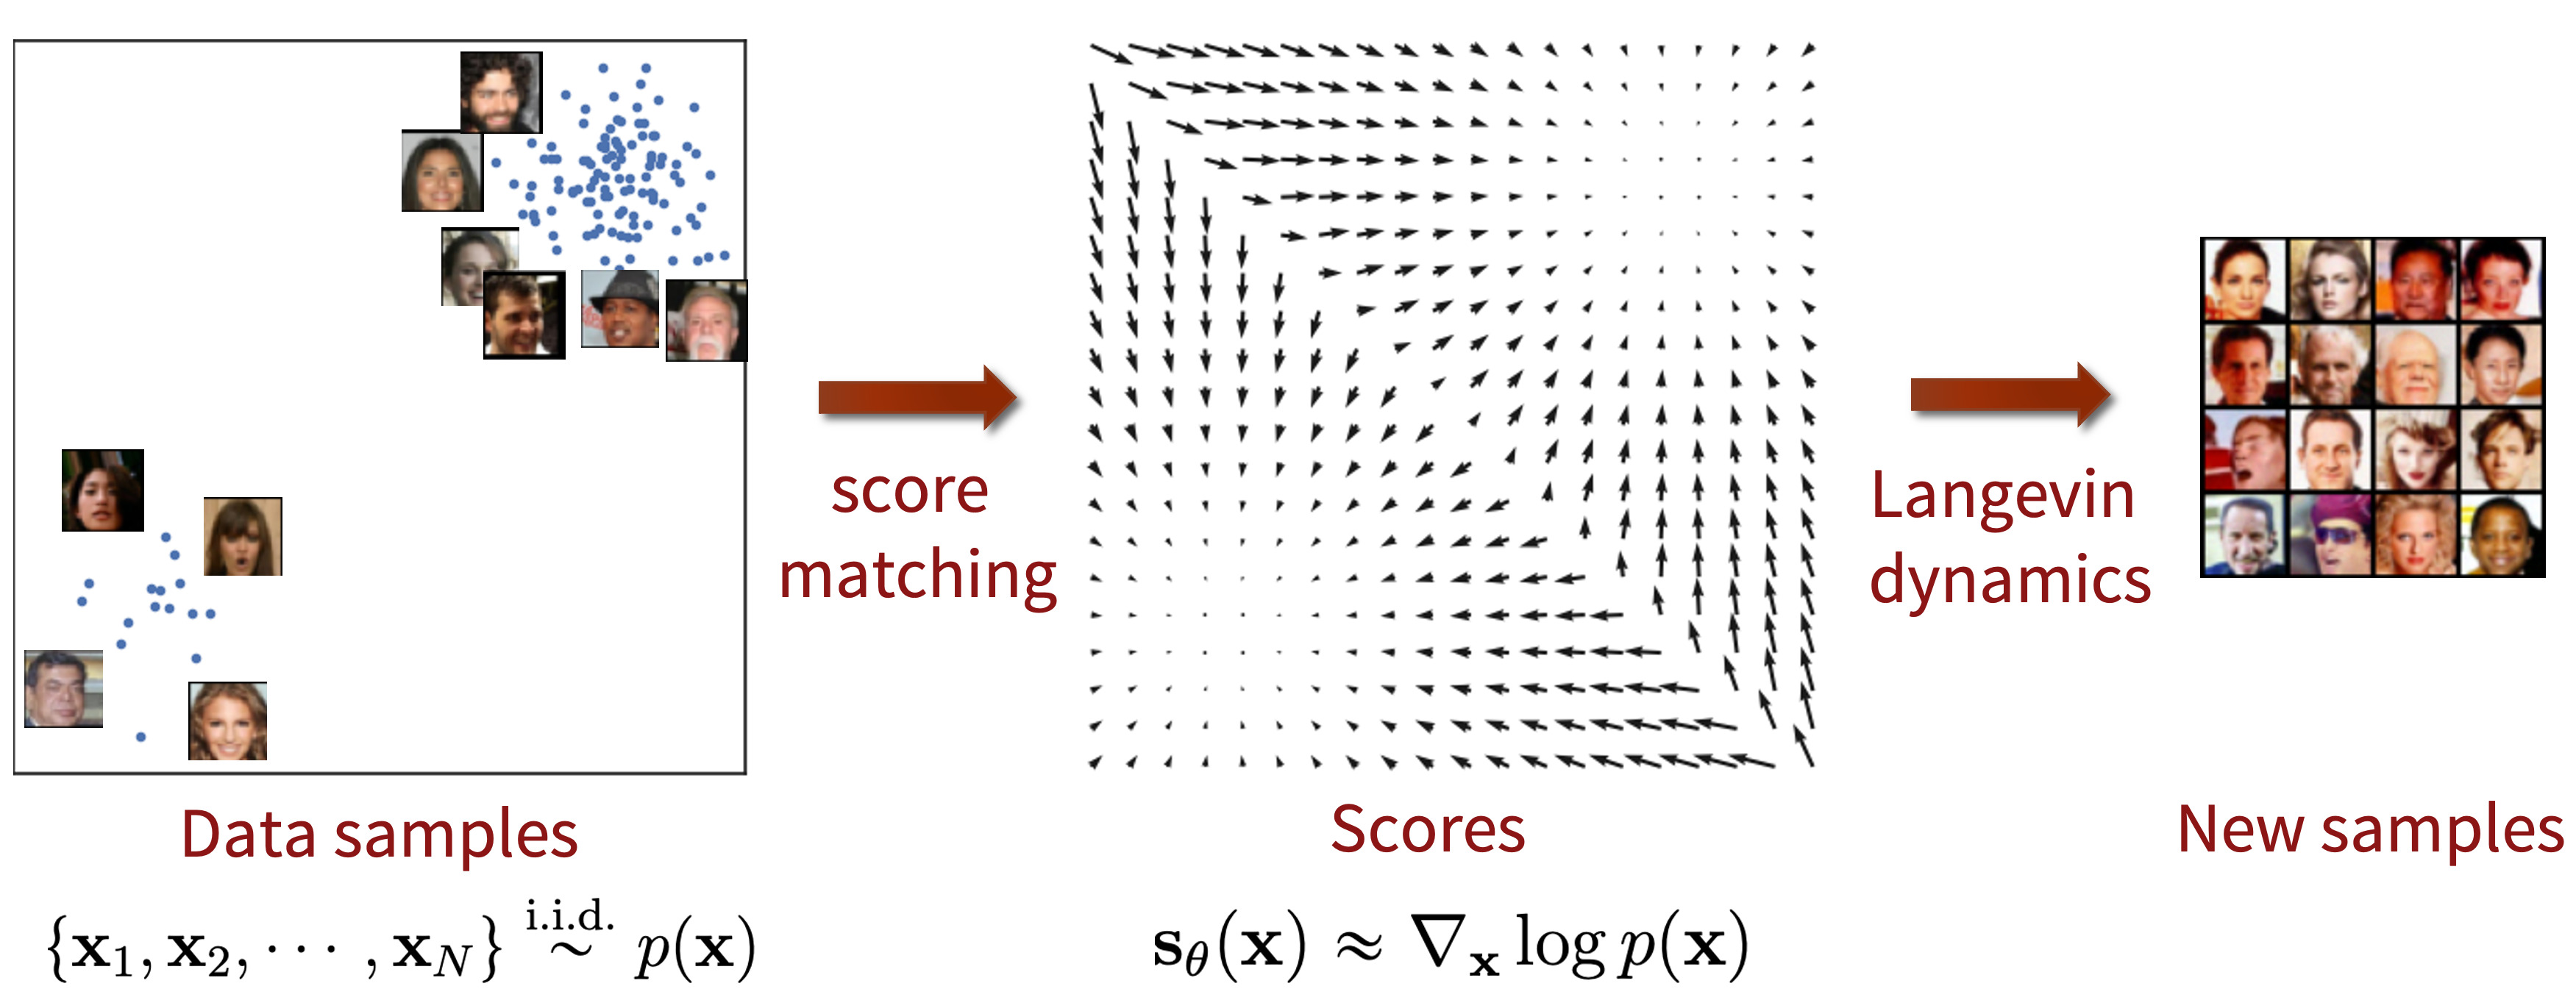
\includegraphics[width=0.75\linewidth]{figs/smld}
	\end{figure}
	\vspace{-0.3cm} 
	\begin{block}{Theorem (implicit score matching)}
		\vspace{-0.6cm}
		\[
		{\color{violet}\frac{1}{2} \bbE_{\pi}\bigl\| \bs_{\btheta}(\bx) - \nabla_\bx \log \pi(\bx) \bigr\|^2_2} = {\color{teal}\bbE_{\pi}\Bigr[ \frac{1}{2}\| \bs_{\btheta}(\bx) \|_2^2 + \text{tr}\bigl(\nabla_{\bx} \bs_{\btheta}(\bx)\bigr) \Bigr]} + \text{const}
		\]
	\end{block}
	\vspace{-0.5cm}
	\begin{enumerate}
		\item {\color{violet}The left hand side} is intractable due to unknown $\pi(\bx)$ -- \textbf{denoising score matching}. 
		\item {\color{teal}The right hand side} is complex due to Hessian matrix -- \textbf{sliced score matching (Hutchinson's trace estimation)}.
	\end{enumerate}
	\myfootnotewithlink{https://yang-song.github.io/blog/2021/score/}{Song Y. Generative Modeling by Estimating Gradients of the Data Distribution, blog post, 2021}
\end{frame}
%=======
\begin{frame}{Recap of previous lecture}
	Let perturb original data by normal noise $p(\bx' | \bx, \sigma) = \cN(\bx' | \bx, \sigma^2 \bI)$
	\vspace{-0.3cm}
	\[
	\pi(\bx' | \sigma) = \int \pi(\bx) p(\bx' | \bx, \sigma) d\bx.
	\]
	\vspace{-0.6cm} \\
	Then the solution of 
	\vspace{-0.2cm}
	\[
	\frac{1}{2} \bbE_{\pi(\bx' | \sigma)}\bigl\| \bs_{\btheta}(\bx', \sigma) - \nabla_{\bx'} \log \pi(\bx' | \sigma) \bigr\|^2_2 \rightarrow \min_{\btheta}
	\]
	\vspace{-0.5cm} \\
	satisfies $\bs_{\btheta}(\bx', \sigma) \approx \bs_{\btheta}(\bx', 0) = \bs_{\btheta}(\bx')$ if $\sigma$ is small enough.
	\begin{block}{Theorem (denoising score matching)}
		\vspace{-0.8cm}
		\begin{multline*}
			\bbE_{\pi(\bx' | \sigma)}\bigl\| \bs_{\btheta}(\bx', \sigma) - \nabla_{\bx'} \log \pi(\bx' | \sigma) \bigr\|^2_2 = \\ = \bbE_{\pi(\bx)} \bbE_{p(\bx' | \bx, \sigma)}\bigl\| \bs_{\btheta}(\bx', \sigma) - \nabla_{\bx'} \log p(\bx' | \bx, \sigma) \bigr\|^2_2 + \text{const}(\btheta)
		\end{multline*}
		\vspace{-0.8cm}
	\end{block}
	Here $\nabla_{\bx'} \log p(\bx' | \bx, \sigma) = - \frac{\bx' - \bx}{\sigma^2}$.
	\begin{itemize}
		\item The RHS does not need to compute $\nabla_{\bx'} \log \pi(\bx' | \sigma)$ and even more $\nabla_{\bx'} \log \pi(\bx')$.
		\item $\bs_{\btheta}(\bx', \sigma)$ tries to \textbf{denoise} a corrupted sample.
		\item Score function $\bs_{\btheta}(\bx', \sigma)$ parametrized by $\sigma$. 
	\end{itemize}
	\myfootnotewithlink{http://www.iro.umontreal.ca/~vincentp/Publications/smdae_techreport.pdf}{Vincent P. A Connection Between Score Matching and Denoising Autoencoders, 2010}
\end{frame}
%=======
\begin{frame}{Recap of previous lecture}
	\begin{block}{Noise conditioned score network}
		\begin{itemize}
			\item Define the sequence of noise levels: $\sigma_1 > \sigma_2 > \dots > \sigma_L$.
			\item Train denoised score function $\bs_{\btheta}(\bx', \sigma)$ for each noise level:
			\vspace{-0.3cm}
			\[
				\sum_{l=1}^L {\color{violet}\sigma_l^2} \bbE_{\pi(\bx)} \bbE_{p(\bx' | \bx, \sigma_l)}\bigl\| \bs_{\btheta}(\bx', \sigma_l) - \nabla_\bx' \log p(\bx' | \bx, \sigma_l) \bigr\|^2_2 \rightarrow \min_{\btheta}
			\]
			\vspace{-0.5cm}
			\item Sample from \textbf{annealed} Langevin dynamics (for $l=1, \dots, L$).
		\end{itemize}
	\end{block}
	\begin{figure}
		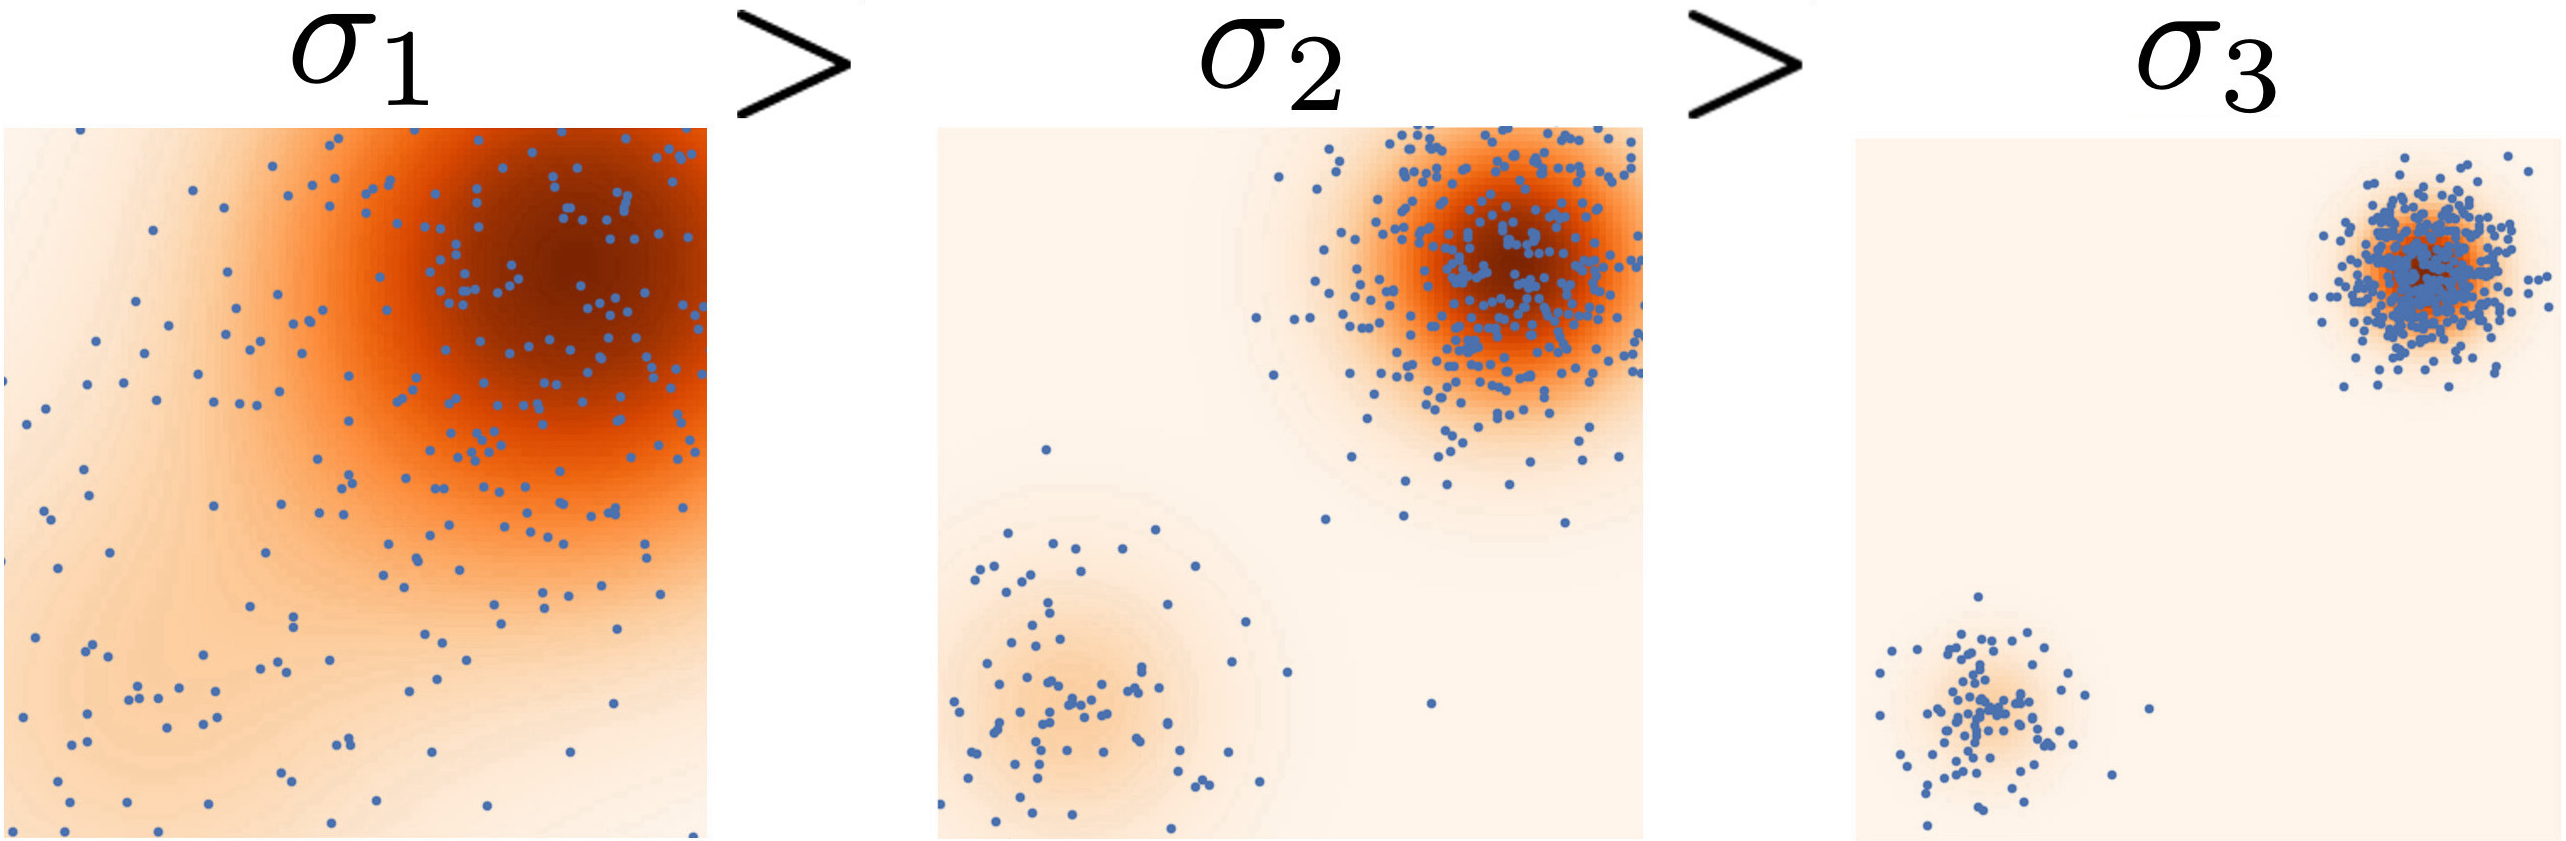
\includegraphics[width=0.55\linewidth]{figs/multi_scale}
	\end{figure}
	\begin{figure}
		
\includegraphics[width=\linewidth]{figs/duoduo}
	\end{figure}
	\myfootnotewithlink{https://arxiv.org/abs/1907.05600}{Song Y. et al. Generative Modeling by Estimating Gradients of the Data Distribution, 2019}
\end{frame}
%=======
\begin{frame}{Recap of previous lecture}
	\begin{block}{NCSN training}
		\begin{enumerate}
			\item Get the sample $\bx_0 \sim \pi(\bx)$.
			\item Sample noise level $l \sim U[1, L]$ and the noise $\bepsilon \sim \cN(0, \bI)$.
			\item Get noisy image $\bx' = \bx_0 + \sigma_l \cdot \bepsilon$.
			\item Compute loss $ \cL = \| \bs_{\btheta}(\bx', \sigma_l) + \frac{\bepsilon}{\sigma_l} \|^2 $.
		\end{enumerate}
	\end{block}
	\begin{block}{NCSN sampling (annealed Langevin dynamics)}
		\begin{itemize}
			\item Sample $\bx_0 \sim \cN(0, \sigma_1 \bI) \approx \pi(\bx | \sigma_1)$.
			\item Apply $T$ steps of Langevin dynamic
			\vspace{-0.2cm}
			\[
				\bx_t = \bx_{t-1} + \frac{1}{2}\eta_l \bs_{\btheta}(\bx_{t - 1}, \sigma_l) + \sqrt{\eta_l} \bepsilon_t.
			\] 
			\vspace{-0.5cm}
			\item Update $\bx_0 := \bx_T$ and choose the next $\sigma_l$.
		\end{itemize}
	\end{block}
	\myfootnotewithlink{https://arxiv.org/abs/2006.09011}{Song Y. et al. Improved Techniques for Training Score-Based Generative Models, 2020}
\end{frame}
%=======
\begin{frame}{Recap of previous lecture}
	\begin{block}{NCSN objective}
		\vspace{-0.2cm}
		\[
			{\color{olive}\bbE_{p(\bx' | \bx, \sigma_l)}}\bigl\| {\color{teal}\bs_{\btheta}(\bx', \sigma_l)} - {\color{violet}\nabla_{\bx'} \log p(\bx' | \bx, \sigma_l)} \bigr\|^2_2 \rightarrow \min_{\btheta}
		\]
	\end{block}
	\vspace{-0.3cm}
	\begin{block}{DDPM objective}
		\vspace{-0.2cm}
		\[
			\cL_t = {\color{olive}\bbE_{\bepsilon \sim \cN(0, \bI)}} \left[ \frac{(1 - \alpha_t)^2}{2\tilde{\beta}_t \alpha_t} \left\| {\color{violet}\frac{\bepsilon}{\sqrt{1 - \bar{\alpha}_t}}} - {\color{teal}\frac{\bepsilon_{\btheta}(\bx_t, t)}{\sqrt{1 - \bar{\alpha}_t}}}\right\|^2 \right]
		\]
		\vspace{-0.7cm}
	\end{block}
	\begin{align*}
		q(\bx_t | \bx_0) &= \cN(\bx_t | \sqrt{\bar{\alpha}_t} \cdot \bx_0, (1 - \bar{\alpha}_t) \cdot \bI) \\
		{\color{violet}\nabla_{\bx_t} \log q(\bx_t | \bx_0)} &= - \frac{\bx_t - \sqrt{\bar{\alpha}_t} \cdot \bx_0}{1 - \bar{\alpha}_t} = - \frac{\bepsilon}{\sqrt{1 - \bar{\alpha}_t}}.
	\end{align*}
		Let reparametrize our model: 
		\vspace{-0.2cm}
		\[
			{\color{teal}\bs_{\btheta}(\bx_t, t)} = - \frac{\bepsilon_{\btheta}(\bx_t, t)}{\sqrt{1 - \bar{\alpha}_t}}.
		\]
	\myfootnotewithlink{https://arxiv.org/abs/2006.11239}{Ho J. Denoising Diffusion Probabilistic Models, 2020}
	\end{frame}
%=======
\begin{frame}{Outline}
	\tableofcontents
\end{frame}
%=======
\section{SDE basics}
%=======
\begin{frame}{Stochastic differential equation (SDE)}
	Let define stochastic process $\bx(t)$ with initial condition $\bx(0) \sim p_0(\bx)$:
	\[
		d\bx = \mathbf{f}(\bx, t) dt + g(t) d \bw
	\]
	\vspace{-0.6cm}
	\begin{itemize}
		 \item $\mathbf{f}(\bx, t)$ is the \textbf{drift} function of $\bx(t)$.
		 \item $g(t)$ is the \textbf{diffusion} coefficient of $\bx(t)$.
		 \item If $g(t) = 0$ we get standard ODE.
		 \item $\bw(t)$ is the standard Wiener process (Brownian motion):
		 \begin{enumerate}
		 	\item $\bw(0) = 0$ (almost surely);
		 	\item $\bw(t)$ has independent increments;
			 \item $\bw(t) - \bw(s) \sim \cN(0, (t - s) \bI)$.
		 \end{enumerate}
		 \item $d \bw = \bw(t + dt) - \bw(t) = \cN(0, \bI \cdot dt ) = \bepsilon \cdot \sqrt{dt}$, where $\bepsilon \sim \cN(0, \bI)$.
	\end{itemize}
	\textbf{Note:} In contrast to ODE, initial condition $\bx(0)$ does not uniquely determine the process trajectory.
\end{frame}
%=======
\begin{frame}{Stochastic differential equation (SDE)}
	\vspace{-0.4cm}
	\[
		d\bx = \mathbf{f}(\bx, t) dt + g(t) d \bw, \quad d \bw = \bepsilon \cdot \sqrt{dt}, \quad \bepsilon \sim \cN(0, \bI).
	\]
	\vspace{-0.4cm}
	\begin{itemize}
		\item At each moment $t$ we have the density $p(\bx(t), t)$.
		\item How to get distribution $p(\bx, t)$ for $\bx(t)$?
	\end{itemize}
 	\begin{block}{Theorem (Kolmogorov-Fokker-Planck)}
 		Evolution of the distribution $p(\bx, t)$ is given by the following ODE:
 		\vspace{-0.2cm}
 		\[
 			\frac{\partial p(\bx, t)}{\partial t} = \text{tr}\left(- \frac{\partial}{\partial \bx} \bigl[ \mathbf{f}(\bx, t) p(\bx, t)\bigr] + \frac{1}{2} g^2(t) \frac{\partial^2 p(\bx, t)}{\partial \bx^2} \right)
 		\]
 		\textbf{Note:} This is the generalization of KFP theorem that we used in continuous-in-time NF.
 	\end{block}
 	\begin{block}{Langevin SDE (special case)}
 		\vspace{-0.6cm}
 		\begin{align*}
 			d\bx &= {\color{violet}\mathbf{f}(\bx, t)} dt + {\color{teal}g(t)} d \bw \\
 			d \bx &= {\color{violet}\frac{1}{2} \frac{\partial}{\partial \bx} \log p(\bx, t)} d t + {\color{teal} 1 } \cdot d \bw
 		\end{align*}
 	\end{block}
\end{frame}
%=======
\begin{frame}{Langevin SDE (special case)}
	\[
		d \bx = {\color{violet}\frac{1}{2} \frac{\partial}{\partial \bx} \log p(\bx, t)} d t + {\color{teal} 1 } \cdot d \bw
	\]
	Let apply KFP theorem.
	\begin{multline*}
		\frac{\partial p(\bx, t)}{\partial t} =  \text{tr} \left(- \frac{\partial}{\partial \bx}\left[ {\color{olive}p(\bx, t) \frac{1}{2} \frac{\partial}{\partial \bx} \log p(\bx, t)} \right]  + \frac{1}{2} \frac{\partial^2 p(\bx, t)}{\partial \bx^2} \right) = \\
		= \text{tr} \left(- \frac{\partial}{\partial \bx}\left[ {\color{olive}\frac{1}{2} \frac{\partial}{\partial \bx} p(\bx, t) } \right]  + \frac{1}{2} \frac{\partial^2 p(\bx, t)}{\partial \bx^2} \right) = 0
	\end{multline*}
	The density $p(\bx, t) = \text{const}(t)$! \\
	\begin{block}{Discretized Langevin SDE}
		\vspace{-0.3cm}
		\[
			\bx_{t + 1} - \bx_t = \eta \frac{1}{2} \frac{\partial}{\partial \bx} \log p(\bx, t) + \sqrt{\eta} \cdot \bepsilon, \quad \eta \approx dt.
		\]
		\vspace{-0.4cm}
	\end{block}
	\begin{block}{Langevin dynamic}
		\vspace{-0.3cm}
		\[
			\bx_{t + 1} = \bx_t + \eta \frac{1}{2} \nabla_{\bx} \log p(\bx | \btheta) + \sqrt{\eta} \cdot \bepsilon, \quad \eta \approx dt.
		\]
		\vspace{-0.3cm}
	\end{block}
\end{frame}
%=======
\section{Diffusion and Score matching SDEs}
%=======
\begin{frame}{Score matching SDE}
	\begin{block}{Denoising score matching}
		\vspace{-0.7cm}
		\begin{align*}
			\bx_l &= \bx + \sigma_l \cdot \bepsilon_l, \quad p(\bx_l | \bx, \sigma_l) = \cN(\bx_l | \bx, \sigma_l^2 \bI) \\
			\bx_{l-1} &= \bx + \sigma_{l-1} \cdot \bepsilon_{l-1}, \quad p(\bx_{l-1} | \bx, \sigma_{l-1}) = \cN(\bx_{l-1} | \bx, \sigma_{l-1}^2 \bI)
		\end{align*}
	\end{block}
	\vspace{-0.7cm}
	\[
		\bx_l = \bx_{l - 1} + \sqrt{\sigma^2_l - \sigma^2_{l-1}} \cdot \bepsilon, \quad p(\bx_l | \bx_{l-1}, \sigma_l) = \cN(\bx_l | \bx_{l-1}, (\sigma_l^2 - \sigma_{l-1}^2) \cdot \bI)
	\]
	Let turn this Markov chain to the continuous stochastic process~$\bx(t)$ taking $L \rightarrow \infty$:
	\[
		{\color{teal}\bx(t + dt)} = {\color{teal}\bx(t)} + \sqrt{\frac{\sigma^2(t + dt) - \sigma^2(t)}{dt} {\color{violet}dt}} \cdot {\color{violet}\bepsilon} = \bx(t) + \sqrt{\frac{ d [\sigma^2(t)]}{dt}} \cdot {\color{violet}d \bw}
	\]
	\vspace{-0.5cm}
	\begin{block}{Variance Exploding SDE}
		\vspace{-0.3cm}
		\[
			d \bx = \sqrt{\frac{ d [\sigma^2(t)]}{dt}} \cdot d \bw
		\]
	\end{block}
	\myfootnotewithlink{https://arxiv.org/abs/2011.13456}{Song Y., et al. Score-Based Generative Modeling through Stochastic Differential Equations, 2020}
\end{frame}
%=======
\begin{frame}{Diffusion SDE}
	\begin{block}{Denoising Diffusion}
		\vspace{-0.5cm}
		\[
			\bx_t = \sqrt{1 - \beta_t} \cdot \bx_{t - 1} + \sqrt{\beta_t} \cdot \bepsilon, \quad q(\bx_t | \bx_{t-1}) = \cN(\bx_t | \sqrt{1 - \beta_t} \cdot \bx_{t-1}, \beta_t \cdot \bI)
		\]
		\vspace{-0.5cm}
	\end{block}
	Let turn this Markov chain to the continuous stochastic process taking $T \rightarrow \infty$ and taking $\beta(\frac{t}{T}) = \beta_t \cdot T$
	\begin{multline*}
		{\color{teal}\bx(t)} = \sqrt{1 - \beta(t) dt} \cdot \bx(t - dt) + \sqrt{\beta(t)dt} \cdot \bepsilon \approx \\
		\approx (1 - \frac{1}{2} \beta(t) dt) \cdot \bx(t - dt) + \sqrt{\beta(t){\color{violet}dt}} \cdot {\color{violet}\bepsilon} = \\
		= {\color{teal}\bx(t - dt)} - \frac{1}{2} \beta(t) \bx(t - dt) dt  + \sqrt{\beta(t)} \cdot {\color{violet}d \bw}
	\end{multline*}
	\vspace{-0.5cm}
	\begin{block}{Variance Preserving SDE}
		\vspace{-0.3cm}
		\[
			{\color{teal}d \bx} = - \frac{1}{2} \beta(t) \bx(t) dt + \sqrt{\beta(t)} \cdot d \bw
		\]
	\end{block}
	\myfootnotewithlink{https://arxiv.org/abs/2011.13456}{Song Y., et al. Score-Based Generative Modeling through Stochastic Differential Equations, 2020}
\end{frame}
%=======
\begin{frame}{Diffusion SDE}
	\begin{figure}
		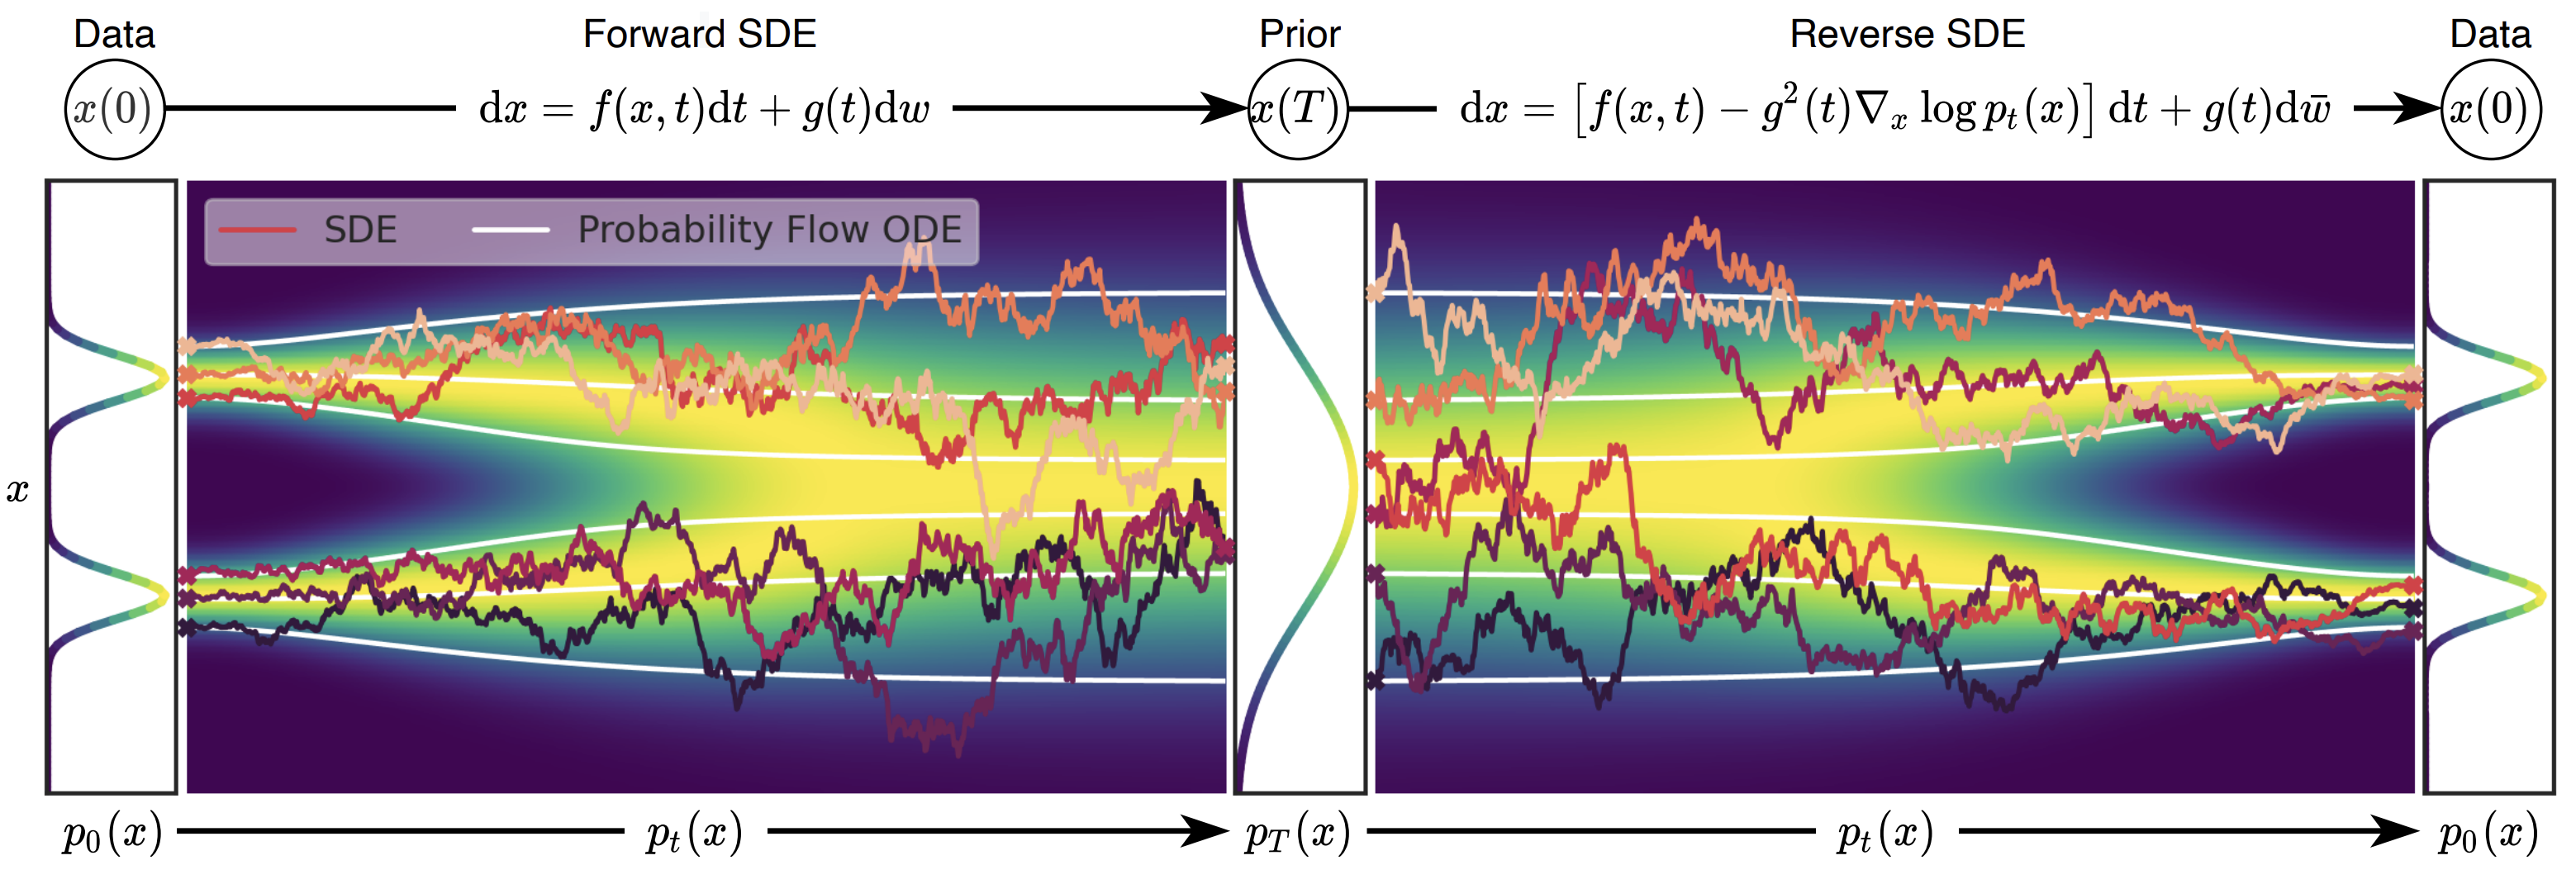
\includegraphics[width=\linewidth]{figs/sde}
	\end{figure}
	\vspace{-0.3cm}
	\begin{block}{Variance Exploding SDE (NCSN)}
		\vspace{-0.3cm}
		\[
			d \bx = \sqrt{\frac{ d [\sigma^2(t)]}{dt}} \cdot d \bw
		\]
		\vspace{-0.3cm}
	\end{block}
	\begin{block}{Variance Preserving SDE (DDPM)}
		\vspace{-0.3cm}
		\[
			d \bx = - \frac{1}{2} \beta(t) \bx(t) dt + \sqrt{\beta(t)} \cdot d \bw
		\]
	\end{block}
	\myfootnotewithlink{https://arxiv.org/abs/2011.13456}{Song Y., et al. Score-Based Generative Modeling through Stochastic Differential Equations, 2020}
\end{frame}
%=======
\section{Guidance}
%=======
\begin{frame}{Guidance}
	\begin{itemize}
	\item Throughout the whole course we have discussed unconditional generative models $p(\bx | \btheta)$.
	\item In practice the majority of the generative models are $\textbf{conditional}$: $p(\bx | \by, \btheta)$.
	\item Here $\by$ could be the class label or $\textbf{text}$ (for text-to-image models).
	\end{itemize}
	\vspace{-0.3cm}
	\begin{minipage}[t]{0.5\columnwidth}
		\begin{figure}
			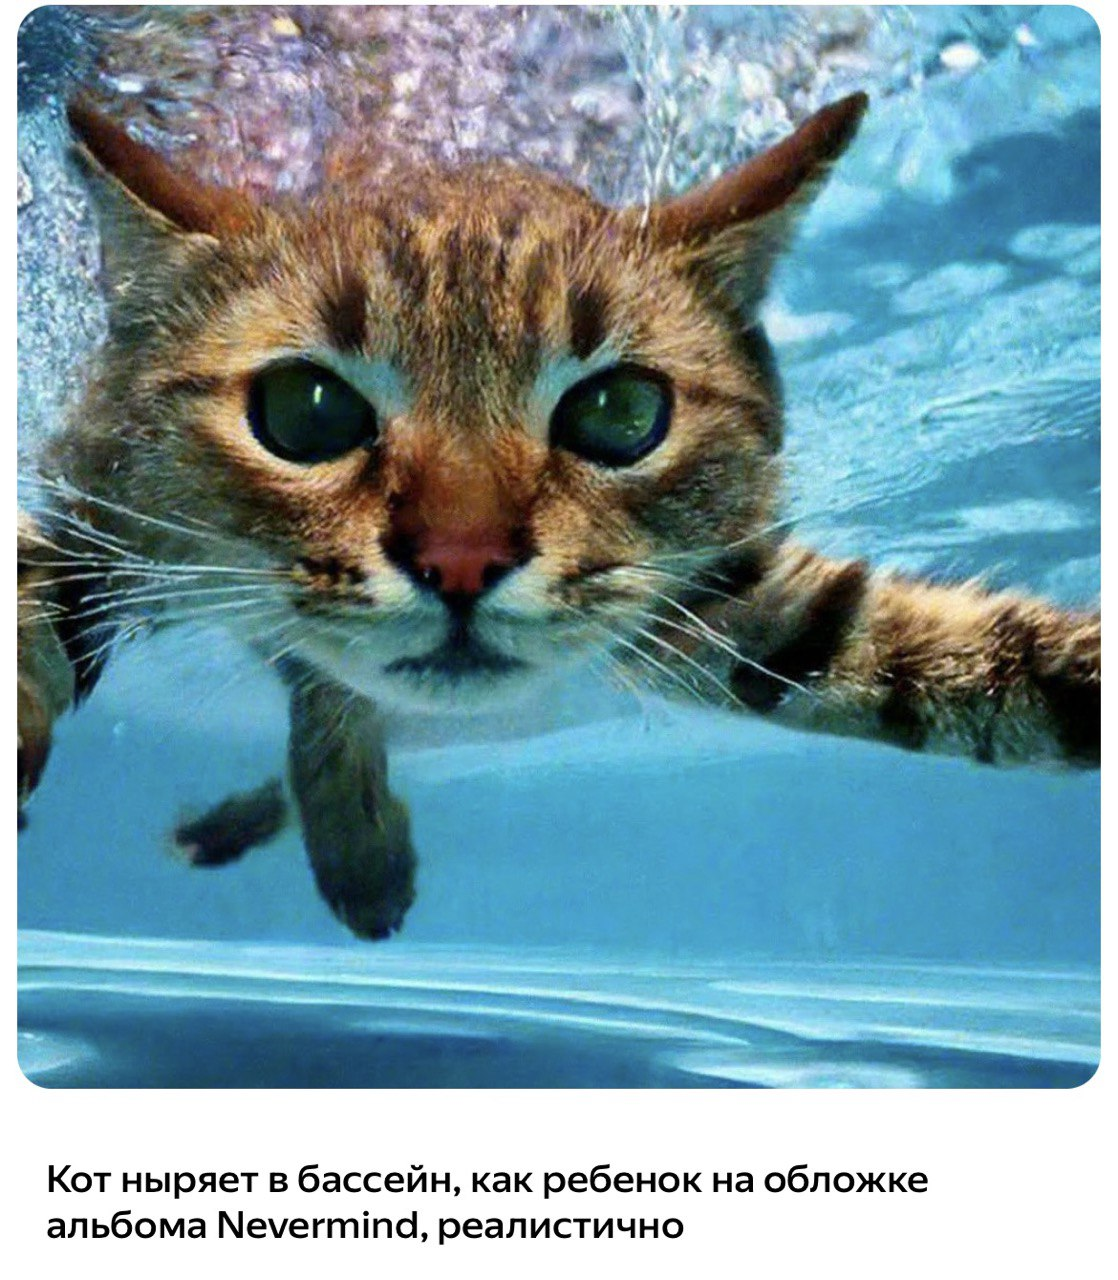
\includegraphics[width=0.9\linewidth]{figs/shedevrum1}
		\end{figure}
	\end{minipage}%
	\begin{minipage}[t]{0.5\columnwidth}
		\begin{figure}
			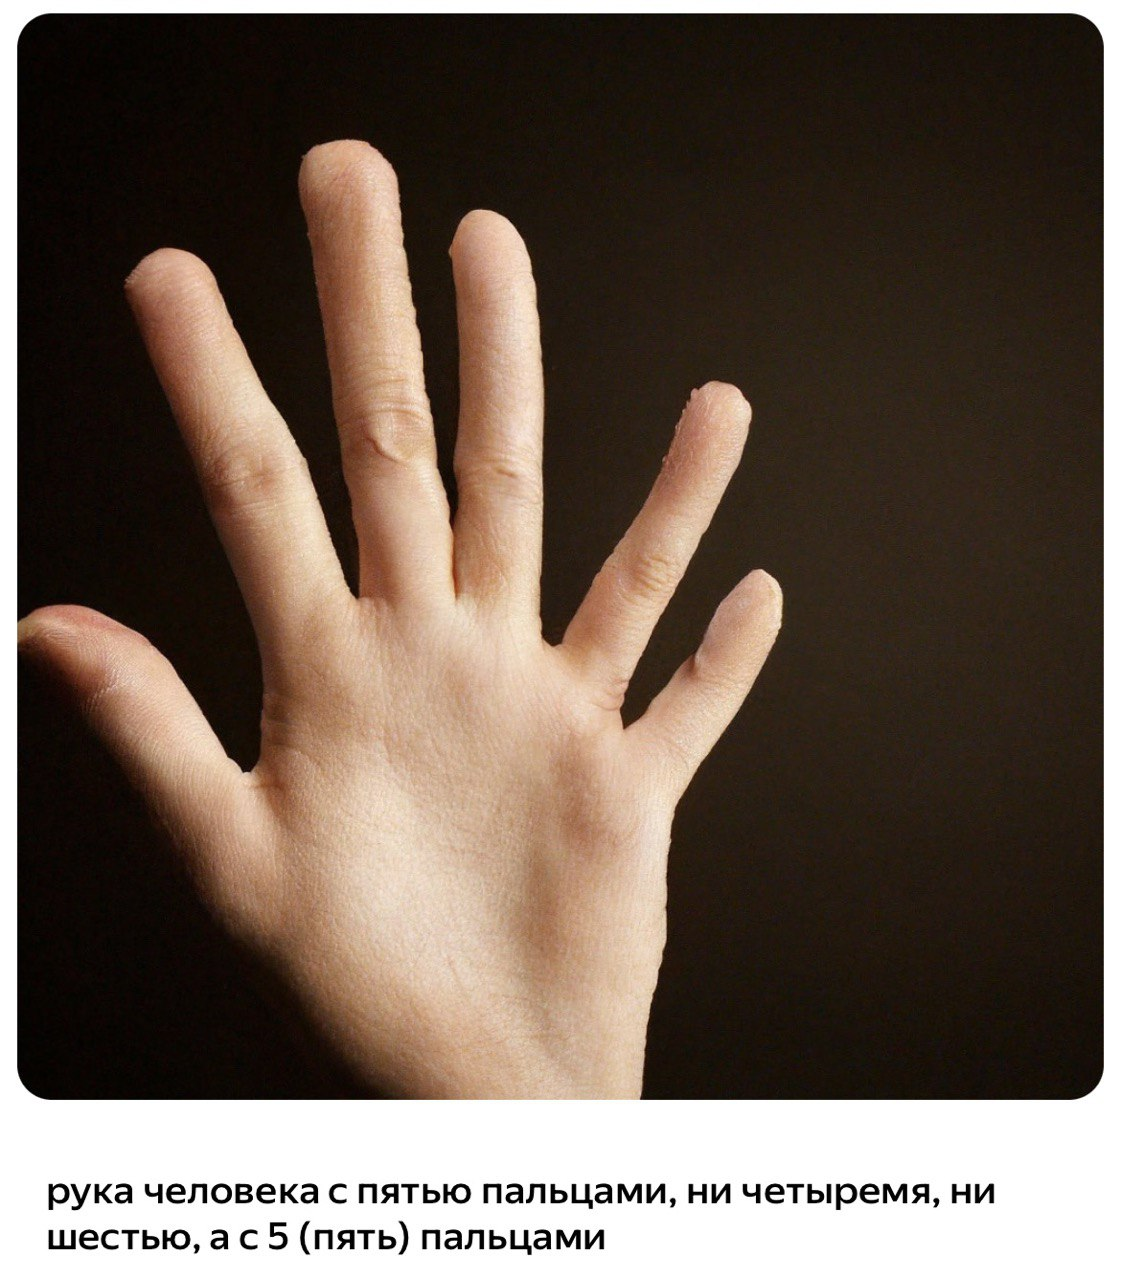
\includegraphics[width=0.9\linewidth]{figs/shedevrum2}
		\end{figure}
	\end{minipage}
\end{frame}
%=======
\begin{frame}{Guidance}
	\begin{block}{How to make conditional model $p(\bx | \by, \btheta)$?}
		\begin{itemize}
		\item If we have \textbf{supervised} data $\{(\bx_i, \by_i)\}_{i=1}^m$ we could theat $\by$ as additional model input:
		\begin{itemize}
			\item $p(x_j | \bx_{1:j-1}, {\color{olive}\by}, \btheta)$ for AR;
			\item Encoder $q(\bz | \bx, {\color{olive}\by}, \bphi)$ and decoder $p(\bx | \bz, {\color{olive}\by}, \btheta)$ for VAE;
			\item $G_{\btheta}(\bz, {\color{olive}\by})$ for NF and GAN;
			\item $p(\bx_{t-1} | \bx_t, {\color{olive}\by}, \btheta)$ for DDPM.
		\end{itemize}
		\item If we have \textbf{unsupervised} data $\{\bx_i\}_{i=1}^m$ we need to create the way to convert unconditional model $p(\bx | \btheta)$ to the conditional.
		\end{itemize}
	\end{block}
	\begin{block}{DDPM \textbf{unsupervised} guidance}
		\begin{itemize}
			\item Let imagine we are given the distribution $q(\by | \bx_0)$. 
			\item Since we have already defined Markov chain, we have $q(\bx_t | \bx_{t-1}, \by) = q(\bx_t | \bx_{t - 1})$.
			\item Let try to find reverse $q(\bx_{t-1} | \bx_t, \by)$.
		\end{itemize}
	\end{block}
\end{frame}
%=======
\begin{frame}{Label guidance}
	\textbf{Label:} Ostrich (10th ImageNet class) 
	\begin{figure}
		\includegraphics[width=\linewidth]{figs/label_conditioning}
	\end{figure}
	\myfootnotewithlink{https://arxiv.org/abs/1906.00446}{Razavi A., Oord A., et al. Generating Diverse High-Fidelity Images with VQ-VAE-2, 2019}
\end{frame}
%=======
\begin{frame}{Text guidance}
	\textbf{Prompt:} a stained glass window of a panda eating bamboo \\
	Left: $\gamma = 1$, Right: $\gamma = 3$.
	\begin{figure}
		\includegraphics[width=\linewidth]{figs/cfg}
	\end{figure}
	\myfootnotewithlink{https://arxiv.org/pdf/2112.10741}{Nichol A., et al. GLIDE: Towards Photorealistic Image Generation and Editing with Text-Guided Diffusion Models, 2022}
\end{frame}
%=======
\subsection{Classifier guidance}
%=======
\begin{frame}{Classifier guidance}
	\vspace{-0.5cm}
	\begin{multline*}
		{\color{teal}q(\by | \bx_{t - 1}, \bx_t)} = \frac{q(\bx_{t - 1}, \bx_t, \by)}{q(\bx_{t - 1}, \bx_t)} = \\
		= \frac{q(\bx_t | \bx_{t - 1}, {\color{olive}\by}) q(\by | \bx_{t - 1}) \color{violet}{q(\bx_{t - 1})}} {q(\bx_t | \bx_{t - 1}) \color{violet}{q(\bx_{t - 1})}} = q(\by | \bx_{t - 1}).
	\end{multline*}
	\vspace{-0.4cm}
	\begin{block}{Conditional distribution}
		\vspace{-0.7cm}
		\begin{multline*}
			q(\bx_{t - 1} | \bx_t, \by) = \frac{q(\bx_{t - 1}, \bx_t, \by)}{q(\bx_t, \by)}  = \\ 
			=  \frac{{\color{teal}q(\by | \bx_{t - 1}, \bx_t)} q(\bx_{t - 1} | \bx_t) {\color{violet}q(\bx_t)}}{q(\by | \bx_t) {\color{violet}q(\bx_t)}} = \\
			= q(\by | \bx_{t - 1}) q(\bx_{t - 1} | \bx_t) \cdot \text{const}(\bx_{t - 1}).
		\end{multline*}
		\[
			p(\bx_{t - 1} | \bx_t, \by, \btheta , \bphi) = p(\by | \bx_{t-1}, \bphi) p(\bx_{t-1} | \bx_t, \btheta) \cdot \text{const}(\bx_{t - 1}).
		\]
		\vspace{-0.4cm}
		\begin{itemize}
			\item $p(\bx_{t-1} | \bx_t, \btheta)$ - our unsupervised diffusion model.
			\item $p(\by | \bx_{t-1}, \bphi)$ - classifier for noised samples $\bx_{t-1}$
		\end{itemize}
	\end{block}
	\myfootnotewithlink{https://arxiv.org/abs/2105.05233}{Dhariwal P., Nichol A. Diffusion Models Beat GANs on Image Synthesis, 2021}
\end{frame}
%=======
\begin{frame}{Classifier guidance}
	\begin{block}{Conditional distribution}
		\vspace{-0.5cm}
		\begin{align*}
			p(\bx_{t - 1} | \bx_t, \by, \btheta , \bphi) &= p(\by | \bx_{t-1}, \bphi) \cdot p(\bx_{t-1} | \bx_t, \btheta) \cdot \text{const}(\bx_{t - 1}) \\
			\log p(\bx_{t - 1} | \bx_t, \by, \btheta , \bphi) &= {\color{teal}\log p(\by | \bx_{t-1}, \bphi)} + {\color{violet}\log p(\bx_{t-1} | \bx_t, \btheta)} + \text{const}
		\end{align*}
	\end{block}
	\vspace{-0.7cm}
	\begin{align*}
		p(\bx_{t-1} | \bx_t, \btheta) &= \cN(\bmu_{\btheta}(\bx_t, t), \bsigma^2_{\btheta}(\bx_t, t)) \\
		{\color{violet}\log p(\bx_{t-1} | \bx_t, \btheta)} &= - \frac{\|\bx_{t - 1} - \bmu\|^2}{2 \bsigma^2} + \text{const}(\bx_{t-1})
	\end{align*}
	\vspace{-0.5cm}
	\begin{block}{Taylor expansion}
		\vspace{-0.7cm}
		\begin{multline*}
			{\color{teal}\log p(\by | \bx_{t-1}, \bphi)} \approx \log p(\by | \bx_{t-1}, \bphi) |_{\bx_{t-1} = \bmu} + \\
			+ (\bx_{t-1} - \bmu) \cdot \nabla_{\bx_{t-1}} \log p(\by | \bx_{t-1}, \bphi) |_{\bx_{t-1} = \bmu} = \\
			= (\bx_{t-1} - \bmu) \cdot \mathbf{g} +  \text{const}(\bx_{t-1}),
		\end{multline*}
		where $\mathbf{g} =  \nabla_{\bx_{t-1}} \log p(\by | \bx_{t-1}, \bphi) |_{\bx_{t-1} = \bmu}$.
	\end{block}
	\myfootnotewithlink{https://arxiv.org/abs/2105.05233}{Dhariwal P., Nichol A. Diffusion Models Beat GANs on Image Synthesis, 2021}
\end{frame}
%=======
\begin{frame}{Classifier guidance}
	\vspace{-0.5cm}
	\begin{align*}
		\log p(\bx_{t - 1} | \bx_t, \by, \btheta , \bphi) &= {\color{teal}(\bx_{t-1} - \bmu) \cdot \mathbf{g}} - {\color{violet}\frac{\|\bx_{t - 1} - \bmu\|^2}{2 \bsigma^2}} + \text{const}(\bx_{t-1}) \\
		& = - \frac{\|\bx_{t - 1} - \bmu - \bsigma \odot \mathbf{g}\|^2}{2 \bsigma^2} + \text{const}(\bx_{t-1}) \\
		& = \log \cN( \bmu + {\color{olive}\bsigma \odot \mathbf{g}}, \bsigma^2) + \text{const}(\bx_{t-1})
	\end{align*}
	\vspace{-0.5cm}
	\begin{block}{Guided sampling}
		\begin{enumerate}
			\item Sample $\bx_T \sim \cN(0, \bI)$.
			\item Compute mean of $p(\bx_{t-1} | \bx_t, \btheta) = \cN(\bmu_{\btheta}(\bx_t, t), \tilde{\beta}_t \bI)$:
			\[
				\bmu_{\btheta}(\bx_t, t) = \frac{1}{\sqrt{\alpha_t}} \bx_t - \frac{1 - \alpha_t}{\sqrt{\alpha_t (1 - \bar{\alpha}_t)}} \cdot \bepsilon_{\btheta}(\bx_t, t).
			\]
			\vspace{-0.3cm}
			\item Compute $\mathbf{g} =  \nabla_{\bx_{t-1}} \log p(\by | \bx_{t-1}, \bphi) |_{\bx_{t-1} = \bmu}$.
			\item Get denoised image $\bx_{t - 1} = (\bmu_{\btheta}(\bx_t, t) +  {\color{olive} \sqrt{\tilde{\beta}_t} \cdot \mathbf{g}})+ \sqrt{\tilde{\beta}_t} \cdot \bepsilon$, where $\bepsilon \sim \cN(0, \bI)$.
		\end{enumerate}
	\end{block}
	\myfootnotewithlink{https://arxiv.org/abs/2105.05233}{Dhariwal P., Nichol A. Diffusion Models Beat GANs on Image Synthesis, 2021}
\end{frame}
%=======
\begin{frame}{Classifier guidance}
	\begin{block}{Theorem (denoising score matching)}
		\vspace{-0.8cm}
		\begin{multline*}
			\bbE_{q(\bx_{t})}\bigl\| \bs_{\btheta}(\bx_t, t) - \nabla_{\bx_t} \log q(\bx_t) \bigr\|^2_2 = \\ = \bbE_{\pi(\bx_0)} \bbE_{q(\bx_t | \bx_0)}\bigl\| \bs_{\btheta}(\bx_t, t) - \nabla_{\bx_t} \log q(\bx_t | \bx_0) \bigr\|^2_2 + \text{const}(\btheta)
		\end{multline*}
		\vspace{-1.0cm}
	\end{block}
	\[
		\nabla_{\bx_t} \log p(\bx_t | \btheta) \approx - \frac{\bepsilon_{\btheta}(\bx_t, t)}{\sqrt{1 - \bar{\alpha}_t}} = \bs_{\btheta}(\bx_t, t).
	\]
	\vspace{-0.4cm}
	\begin{block}{Conditional distribution}
		\vspace{-0.7cm}
		\begin{align*}
			{\color{olive}\nabla_{\bx_t} \log p(\bx_t | \by, \btheta, \bphi)} &= \nabla_{\bx_t} \log \left(\frac{p(\by | \bx_t, \bphi)p(\bx_t | \btheta)}{p(\by | \bphi)} \right)\\
			&= \nabla_{\bx_t} \log p(\by | \bx_t, \bphi) + {\color{violet}\nabla_{\bx_t} \log p(\bx_t | \btheta)}\\
			&= {\color{teal}\nabla_{\bx_t} \log p(\by | \bx_t, \bphi)} {\color{violet}- \frac{\bepsilon_{\btheta}(\bx_t, t)}{\sqrt{1 - \bar{\alpha}_t}}}
		\end{align*}
		\vspace{-0.7cm}
	\end{block}
	\begin{block}{Classifier-corrected noise prediction}
		\vspace{-0.4cm}
		\[
			{\color{olive}\hat{\bepsilon}_{\btheta}(\bx_t, t)} = {\color{violet}\bepsilon_{\btheta}(\bx_t, t)} - {\color{violet}\sqrt{1 - \bar{\alpha}_t}} \cdot {\color{teal}\nabla_{\bx_t} \log p(\by | \bx_t, \bphi)}
		\]
	\end{block}
	\myfootnotewithlink{https://arxiv.org/abs/2105.05233}{Dhariwal P., Nichol A. Diffusion Models Beat GANs on Image Synthesis, 2021}
\end{frame}
%=======
\begin{frame}{Classifier guidance}
	\begin{block}{Classifier-corrected noise prediction}
		\vspace{-0.7cm}
		\begin{align*}
			\hat{\bepsilon}_{\btheta}(\bx_t, t) &= \bepsilon_{\btheta}(\bx_t, t) - \sqrt{1 - \bar{\alpha}_t} \cdot \nabla_{\bx_t} \log p(\by | \bx_t, \bphi) \\
			\hat{\bepsilon}_{\btheta}(\bx_t, t) &= \bepsilon_{\btheta}(\bx_t, t) - {\color{teal}\gamma} \cdot \sqrt{1 - \bar{\alpha}_t} \cdot \nabla_{\bx_t} \log p(\by | \bx_t, \bphi)
		\end{align*}
		\vspace{-0.7cm}
	\end{block}
	Here we introduce {\color{teal} guidance scale $\gamma$} that controls the magnitude of the classifier guidance.
	\begin{block}{Conditional distribution}
		\vspace{-0.2cm}
		\[
			\frac{\hat{\bepsilon}_{\btheta}(\bx_t, t)}{\sqrt{1 - \bar{\alpha}_t}} = \frac{\bepsilon_{\btheta}(\bx_t, t)}{\sqrt{1 - \bar{\alpha}_t}} - {\color{teal}\gamma} \cdot \nabla_{\bx_t} \log p(\by | \bx_t, \bphi)
		\]
		\vspace{-0.5cm}
		\begin{align*}
			\nabla_{\bx_t}^{\gamma} \log p(\bx_t | \by, \btheta, \bphi) &= \gamma \cdot \nabla_{\bx_t} \log p(\by | \bx_t, \bphi) + \nabla_{\bx_t} \log p(\bx_t | \btheta) \\
			p(\bx_t | \by, \btheta, \bphi) &= \frac{p(\by | \bx_t, \bphi)^{\gamma} p(\bx_t | \btheta)}{Z}
		\end{align*}
		\vspace{-0.5cm}
	\end{block}
	Check that $\nabla_{\bx_t} \log Z \neq 0$.
	\myfootnotewithlink{https://arxiv.org/abs/2105.05233}{Dhariwal P., Nichol A. Diffusion Models Beat GANs on Image Synthesis, 2021}
\end{frame}
%=======
\begin{frame}{Classifier guidance}
	\begin{block}{Guided sampling}
		\begin{enumerate}
			\item Sample $\bx_T \sim \cN(0, \bI)$.
			\item Compute "corrected" $\hat{\bepsilon}_{\btheta}(\bx_t, t)$:
			\[
				{\color{olive}\hat{\bepsilon}_{\btheta}(\bx_t, t)} = \bepsilon_{\btheta}(\bx_t, t) - {\color{teal}\gamma} \cdot \sqrt{1 - \bar{\alpha}_t} \cdot \nabla_{\bx_t} \log p(\by | \bx_t, \bphi)
			\]
			\item Compute mean of $p(\bx_{t-1} | \bx_t, \btheta) = \cN(\bmu_{\btheta}(\bx_t, t), \tilde{\beta}_t \bI)$:
			\[
				\bmu_{\btheta}(\bx_t, t) = \frac{1}{\sqrt{\alpha_t}} \bx_t - \frac{1 - \alpha_t}{\sqrt{\alpha_t (1 - \bar{\alpha}_t)}} \cdot  	{\color{olive}\hat{\bepsilon}_{\btheta}(\bx_t, t)}
			\]
			\vspace{-0.3cm}
			\item Get denoised image $\bx_{t - 1} = \bmu_{\btheta}(\bx_t, t) +  \sqrt{\tilde{\beta}_t} \cdot \bepsilon$, where $\bepsilon \sim \cN(0, \bI)$.
		\end{enumerate}
	\end{block}
	\myfootnotewithlink{https://arxiv.org/abs/2105.05233}{Dhariwal P., Nichol A. Diffusion Models Beat GANs on Image Synthesis, 2021}
\end{frame}
%=======
\subsection{Classifier-free guidance}
%=======
\begin{frame}{Classifier-free guidance}
	Previous methods require training the additional classifier model $p(\by | \bx_t, \btheta)$ on the noisy data.
	Let try to avoid this requirement.
	\vspace{-0.3cm}
	\begin{multline*}
		\nabla_{\bx_t}^{\gamma} \log p(\bx_t | \by, \btheta, \bphi) = \gamma \cdot \nabla_{\bx_t} {\color{violet}\log p(\by | \bx_t, \bphi)} + \nabla_{\bx_t} \log p(\bx_t | \btheta) = \\
		= \gamma \cdot  \nabla_{\bx_t} \log \left( {\color{violet}\frac{p(\bx_t| \by, \btheta, \bphi) p(\by | \bphi)}{p(\bx_t | \btheta)}} \right) + \nabla_{\bx_t} \log p(\bx_t | \btheta) = \\
		= \gamma \cdot  \nabla_{\bx_t} \log p(\bx_t| \by, \btheta, \bphi) -\gamma \cdot  \nabla_{\bx_t} \log  p(\bx_t | \btheta) + \nabla_{\bx_t} \log p(\bx_t | \btheta) = \\
		= \gamma \cdot  \nabla_{\bx_t} \log p(\bx_t| \by, \btheta, \bphi) + (1 - \gamma) \cdot  \nabla_{\bx_t} \log p(\bx_t | \btheta)
	\end{multline*}
	What will we get if $\gamma = 1$?
	\begin{block}{Classifier-free-corrected noise prediction}
		\vspace{-0.3cm}
		\[
			\hat{\bepsilon}_{\btheta}(\bx_t, t) = \gamma \cdot \bepsilon_{\btheta}(\bx_t, \by, t) + (1 - \gamma) \cdot \bepsilon_{\btheta}(\bx_t, t)
		\]
		\vspace{-0.5cm}
	\end{block}
	In practice we could train the single model $\bepsilon_{\btheta}(\bx_t, \by, t)$ on \textbf{supervised} data alternating with real conditioning $\by$ and empty conditioning $\by = \emptyset$.
	\myfootnotewithlink{https://arxiv.org/abs/2207.12598}{Ho J., Salimans T. Classifier-Free Diffusion Guidance, 2022}
\end{frame}
%=======
\section{The worst course overview}
%=======
\begin{frame}{The worst course overview :)}
	\begin{figure}
		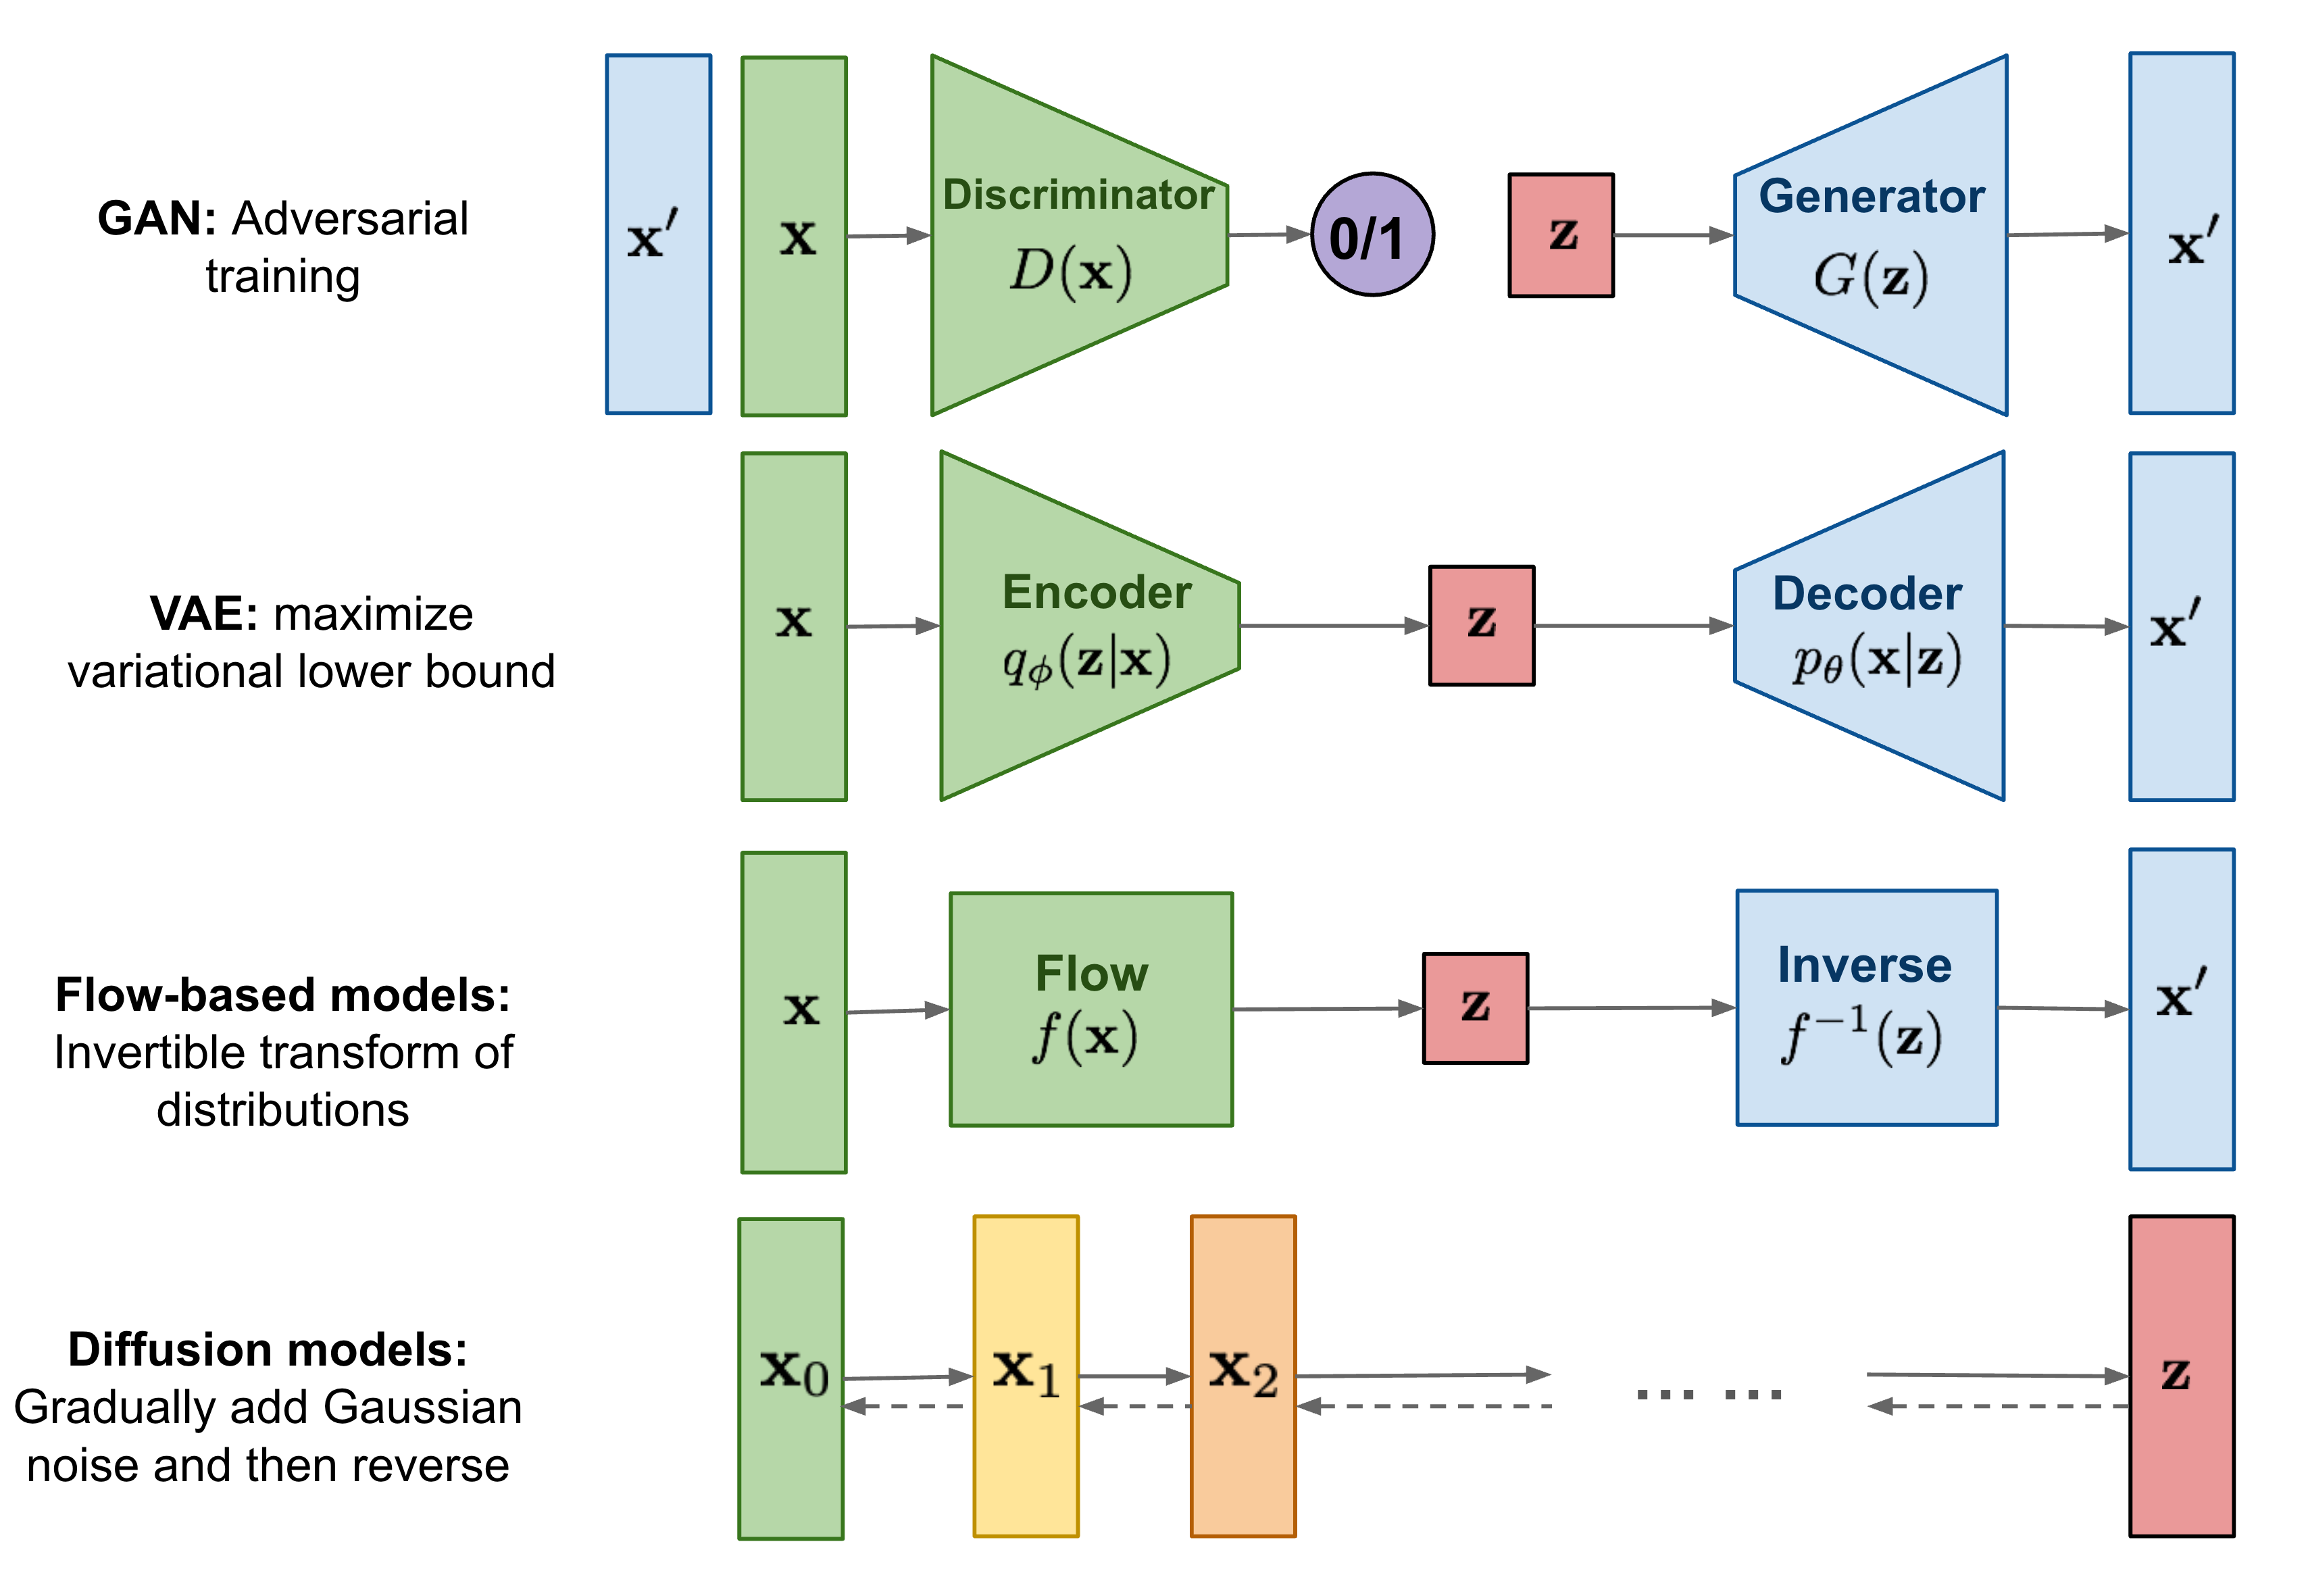
\includegraphics[width=\linewidth]{figs/generative-overview}
	\end{figure}
	\myfootnotewithlink{https://lilianweng.github.io/posts/2021-07-11-diffusion-models/}{Weng L. What are Diffusion Models?, blog post, 2021}
\end{frame}
%=======
\begin{frame}{The worst course overview :)}
	\begin{figure}
		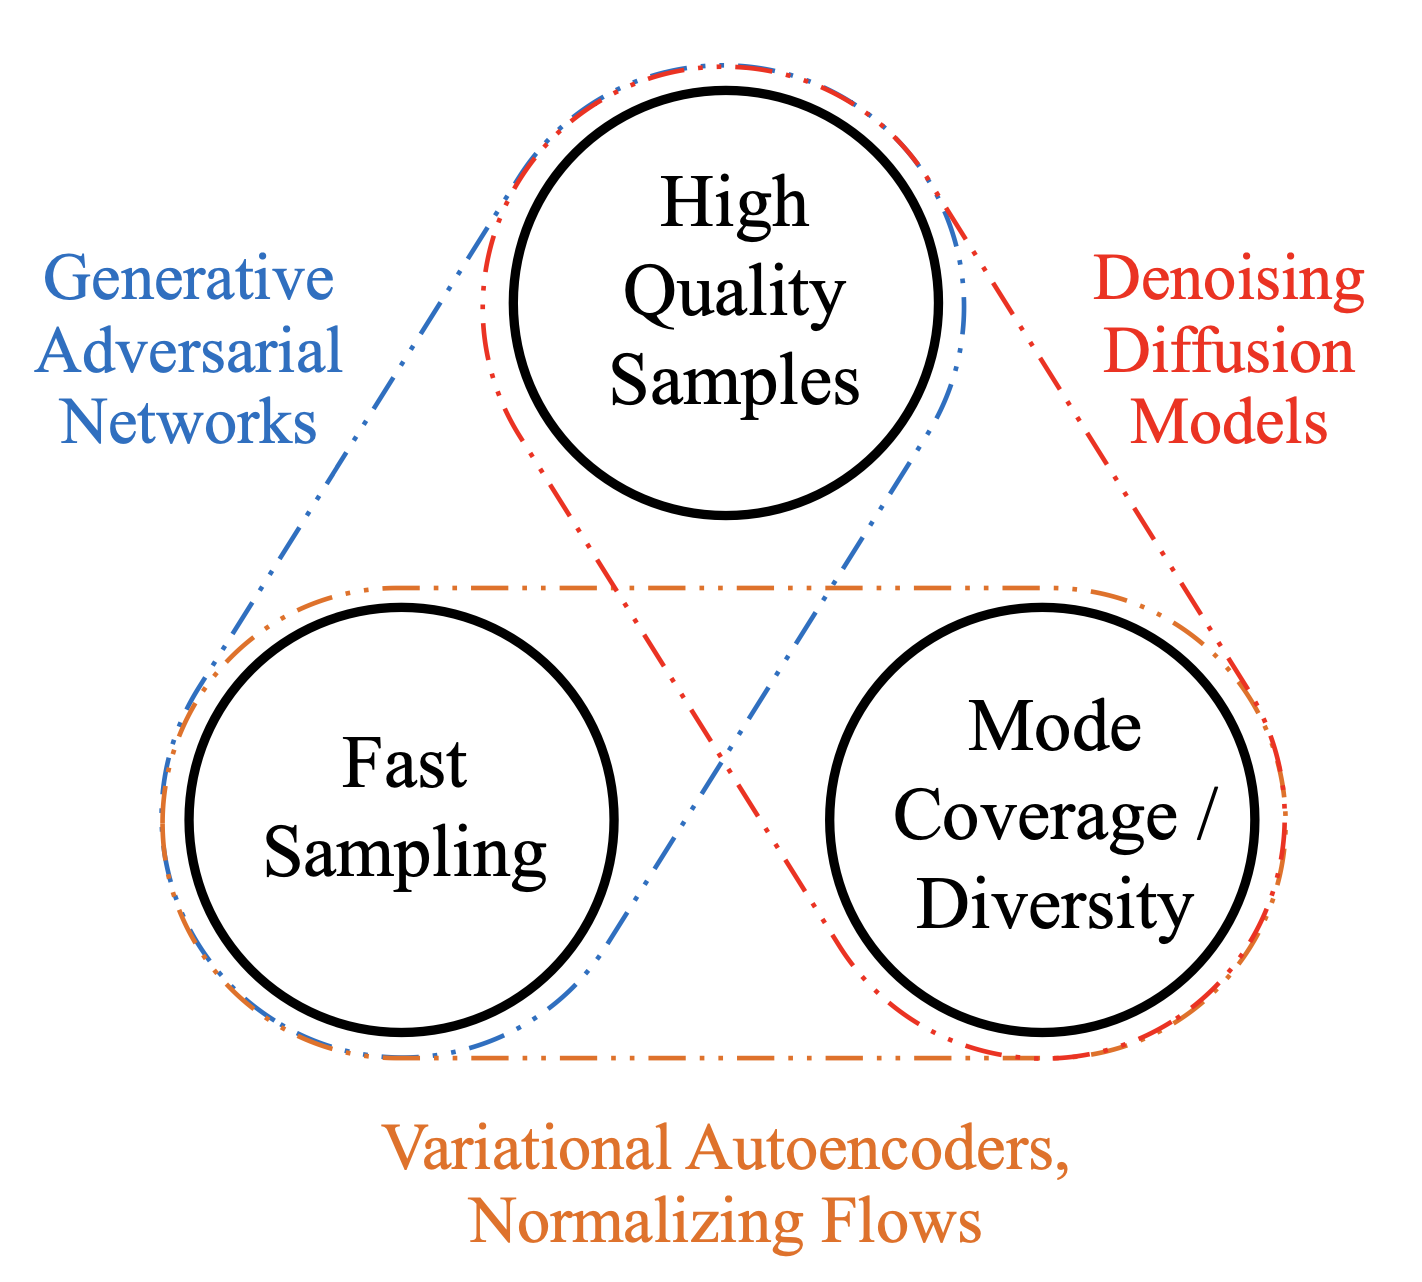
\includegraphics[width=0.7\linewidth]{figs/trilemma}
	\end{figure}
	\myfootnotewithlink{https://arxiv.org/abs/2112.07804}{Xiao Z., Kreis K., Vahdat A. Tackling the generative learning trilemma with denoising diffusion GANs, 2021}
\end{frame}
%=======
\begin{frame}{The worst course overview :)}
	\begin{figure}
		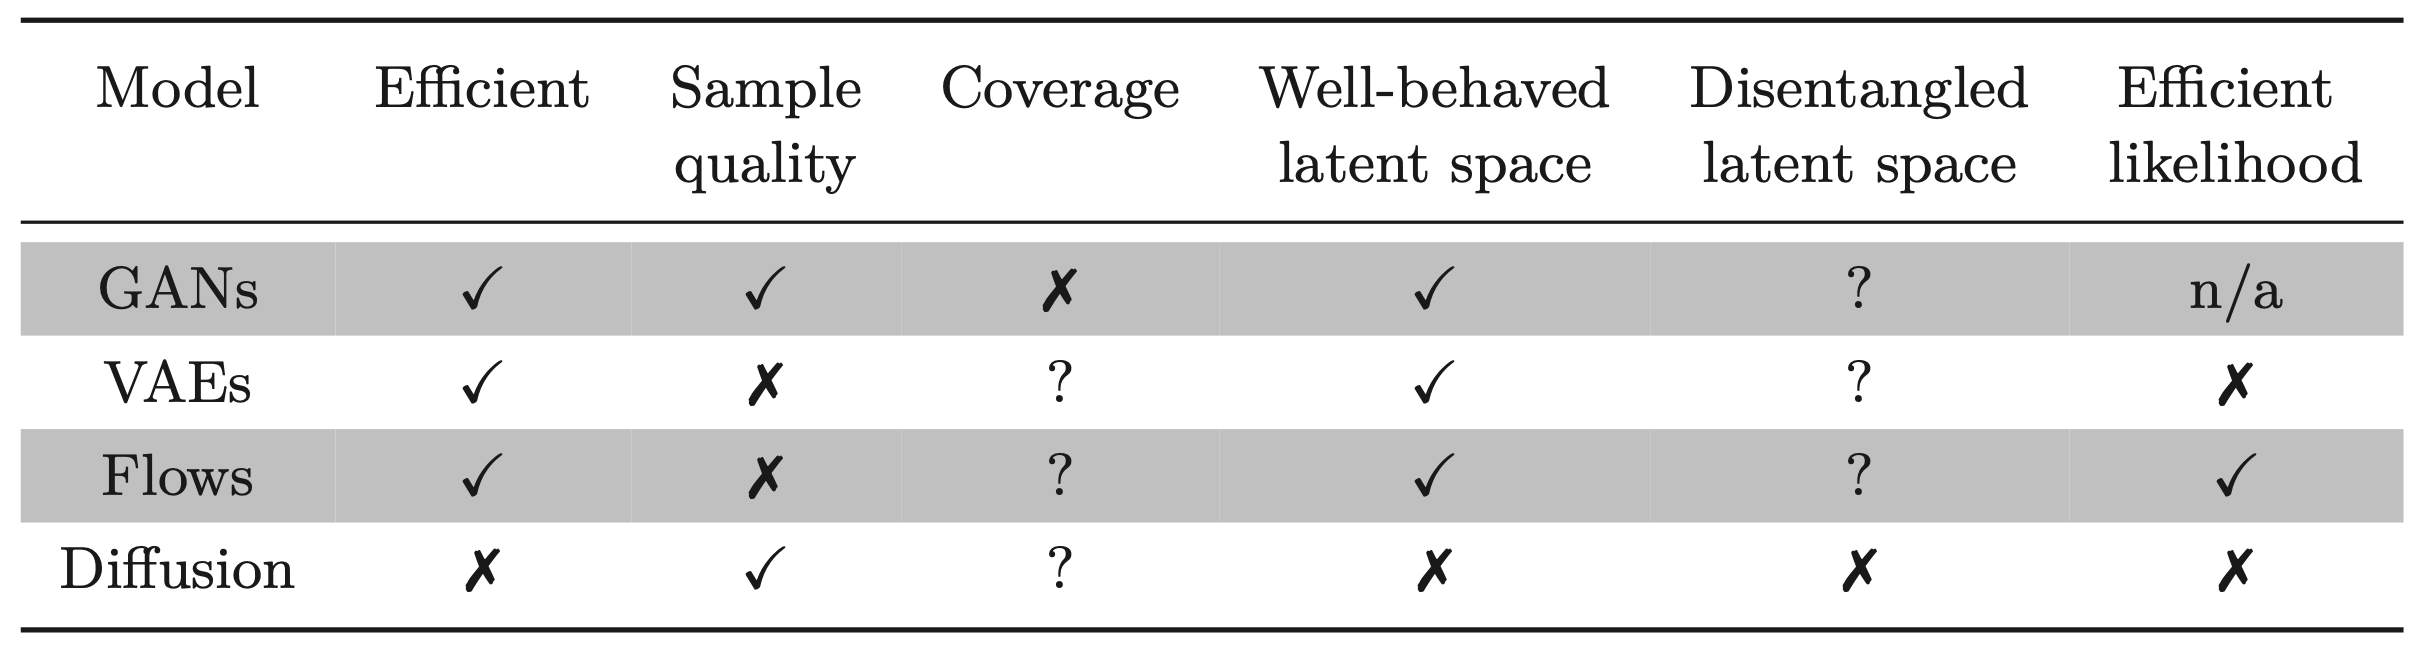
\includegraphics[width=\linewidth]{figs/gen_comp_table}
	\end{figure}
	\myfootnotewithlink{https://udlbook.github.io/udlbook/}{Simon J.D. Prince. Understanding Deep Learning, 2023}
\end{frame}
%=======
\begin{frame}{Summary}
	\begin{itemize}
		\item Score matching (NCSN) and diffusion models (DDPM) are the discretizations of the SDEs (variance exploding and variance preserving).
		\vfill
		\item Conditional models use labels $\by$ as the additional input. Majority of the modern generative models are conditional.
		\vfill
		\item Classifier guidance is the way to turn the unconditional model to the conditional one via the training additional classifier on the noisy data.
		\vfill
		\item Classifier-free guidance allows to avoid the training additional classifier to get the conditional model. It is widely used in practice.
	\end{itemize}
\end{frame}
\end{document} 